% !TEX encoding = UTF-8 Unicode
% !TEX TS-program = xelatex
% !BIB program = biber

% MIT License
%
% Copyright (c) 2019 Star Brilliant
%
% Permission is hereby granted, free of charge, to any person obtaining a copy
% of this software and associated documentation files (the "Software"), to deal
% in the Software without restriction, including without limitation the rights
% to use, copy, modify, merge, publish, distribute, sublicense, and/or sell
% copies of the Software, and to permit persons to whom the Software is
% furnished to do so, subject to the following conditions:
%
% The above copyright notice and this permission notice shall be included in
% all copies or substantial portions of the Software.
%
% THE SOFTWARE IS PROVIDED "AS IS", WITHOUT WARRANTY OF ANY KIND, EXPRESS OR
% IMPLIED, INCLUDING BUT NOT LIMITED TO THE WARRANTIES OF MERCHANTABILITY,
% FITNESS FOR A PARTICULAR PURPOSE AND NONINFRINGEMENT. IN NO EVENT SHALL THE
% AUTHORS OR COPYRIGHT HOLDERS BE LIABLE FOR ANY CLAIM, DAMAGES OR OTHER
% LIABILITY, WHETHER IN AN ACTION OF CONTRACT, TORT OR OTHERWISE, ARISING FROM,
% OUT OF OR IN CONNECTION WITH THE SOFTWARE OR THE USE OR OTHER DEALINGS IN THE
% SOFTWARE.

\documentclass{HDU-Bachelor-Thesis}

% 导入 \addbibresource \printbibliography
\usepackage{biblatex}
% 导入 \includepdf
\usepackage{pdfpages}
% 导入 \sout
\usepackage{ulem}
% 导入 \setmathfont
\usepackage{unicode-math}
% 导入 \textcolor
\usepackage{xcolor}
% 导入 图片的宏包
\usepackage{graphicx}
% 导入 设置图片浮动位置的宏包
\usepackage{float}
% 导入 多图时用子图显示的宏包
\usepackage{subfigure}
% 修改 \begin{enumerate} 间距
\usepackage{paralist}

\setcounter{secnumdepth}{4}
% \setcounter{tocdepth}{4}

\let\itemize\compactitem
\let\enditemize\endcompactitem
\let\enumerate\compactenum
\let\endenumerate\endcompactenum
\let\description\compactdesc
\let\enddescription\endcompactdesc

% 图表前缀配置
\renewcommand {\thetable} {\thesection{}-\arabic{table}}
\renewcommand {\thefigure} {\thesection{}-\arabic{figure}}

\title{基于容器化技术的机器学习运维自动化系统}
\author{肖良玉}
\date{2023 年 6 月 5 日}
\HDUyear{2023}
\HDUschool{计算机学院}
\HDUmajor{计算机科学与技术}
\HDUclassid{19052321}
\HDUstudentid{19194125}
\HDUadviser{陈溪源}
\HDUfinishdate{2023 年 6 月}
\HDUsigndate{2023 年 6 月 5 日}

% 从 ref.bib 中读入参考文献
\addbibresource{ref.bib}

% 设置公式字体(其它字体在模板中已设置好)
\setmathfont{texgyretermes-math.otf}

\begin{document}
% 页码在 PDF 阅读器中显示为罗马数字
\pagenumbering{roman}
% 关闭页眉、页脚
\pagestyle{empty}

% 生成封面
\maketitle
% 或者使用 Microsoft Word 制作封面后导入
%\includepdf[pages={-}]{封面.pdf}

\clearpage
% 关闭页脚
% \pagestyle{HDU-bachelor-empty}

\section*{摘\hspace{2em}要}

本论文设计并实现了一套MLOps(机器学习运维自动化)系统。MLOps系统致力于加速机器学习模型从开发到生产的部署过程,提高模型的可靠性和生产力。论文详细描述了实现该MLOps系统的技术架构和流程。MLOps是一种新的工程实践,其旨在将机器学习模型高效地从开发过程转移到生产过程,为企业快速满足市场需求,提高机器学习模型在生产环境中的可靠性提供支持。本文探究了MLOps实现的关键,其中容器化技术,特别是Docker等工具的支持发挥了重要作用。本论文详细介绍了MLOps的全流程,包括模型上传、模型部署、API自动生成、API测试与优化以及API发布与维护等步骤。

论文采用Docker等容器技术,实现了模型的容器化部署和管理。论文设计了一套CI/CD流水线,实现了模型镜像的自动化构建、测试和部署。该项目使用GitHub Action完成模型的自动化构建和测试,并自动将测试通过的模型推送到Docker Hub。然后,该项目设计了web后台,可以在后台填入Docker Hub中模型的URL,实现模型的自动化部署。

本MLOps系统具有广泛的应用前景。它不但可以应用于企业内部,实现自动化的机器学习模型开发与部署,还可以对外提供机器学习模型服务,为企业创造更高价值。

总之,本论文设计并实现了一套完整的MLOps系统,采用先进的容器和DevOps技术,实现了机器学习模型从开发到生产的自动化流程管理。

\vspace{\baselineskip}\noindent
\textsf{关键词:}机器学习运维自动化;容器化;Docker;机器学习;后端

\clearpage
\section*{\textbf{ABSTRACT}}

This paper designs and implements a machine learning operations (MLOps) system. The MLOps system is dedicated to accelerating the deployment process of machine learning models from development to production, and improving the reliability and productivity of the models. The paper describes the technical architecture and process for implementing the MLOps system in detail. MLOps is a new engineering practice that aims to efficiently transfer machine learning models from development to production, to support enterprises in quickly meeting market demand, and to improve the reliability of machine learning models in production environments. This paper explores the key factors in implementing MLOps, with containerization technology, especially Docker and other tools, playing an important role. The paper also provides a detailed introduction to the complete process of MLOps, including model uploading, deployment, API auto-generation, API testing and optimization, and API publishing and maintenance.

The paper uses container technology such as Docker to implement model containerization deployment and management. A CI/CD pipeline is designed to achieve automatic image construction, testing, and deployment of the model. The project uses GitHub Action to automatically build and test models, and pushes the tested model to Docker Hub. Then, the project is designed with a web backend to automatically deploy the model by filling in the URL of the model in Docker Hub.

This MLOps system has a wide range of application prospects. It can not only be used for automated machine learning model development and deployment within an enterprise, but also provide machine learning model services externally, creating higher value for the enterprise.

In summary, this paper designs and implements a complete MLOps system, using advanced container and DevOps technology to achieve automated process management of machine learning models from development to production.

\vspace{\baselineskip}\noindent
\textbf{Key words:} MLOps;Container Technology;Docker;Machine Learning;Backend

\clearpage
% 生成目录
\tableofcontents
\clearpage

\listoffigures
\listoftables

\clearpage
% 将页码重置为 1
\pagenumbering{arabic}
% 开启页脚
% \pagestyle{HDU-bachelor}

\section{引言}

目前的机器学习模型部署与服务化过程主要依靠人工操作完成,开发成本高,部署效率低。传统的部署方式无法实现自动化、标准化和规模化。因此有必要设计一套机器学习运维自动化系统,这样既能保证模型快速迭代更新,又能实现规模化服务,具有重大的实用价值。

近年来,容器技术和云原生技术日益发展,为机器学习系统的自动化、规模化部署提供了技术基础。本设计采用容器化与DevOps理念,具有自动化、轻量级、规模化等特征。该系统主要从三个方面实现机器学习系统的CI/CD:

首先,系统集成了GitHub Action,用于实现代码提交后的持续集成。开发人员只需要在代码仓库中配置YAML文件,即可完成单元测试、静态代码检测、构建Docker镜像等流程。当代码提交或合并请求触发Action时,系统会自动拉取最新代码并执行配置的任务,若通过检查则生成Docker镜像。

其次,系统实现了镜像的自动构建和推送。Docker镜像构建完成后,会自动推送到Docker Hub公共仓库中,此过程不需要人工干预。开发人员可以在任何地方随时拉取需要的镜像来部署服务。

最后,系统设计了一个Web界面用于服务部署。在部署页面可以选择Docker Hub中的镜像并填入服务器节点IP,系统会自动在目标服务器上部署服务,包括拉取镜像、资源分配、环境变量配置、性能监控等。

总之,该系统基于当前主流技术,设计一套机器学习的CI/CD系统,能够实现模型从开发到部署的全流程自动化。具有自动化、轻量级、规模化等特征,可以大幅降低模型部署的人工成本,实现快速更新迭代,具有重要的理论研究价值和实践应用前景。

该设计通过Docker等容器化技术以及Git、GitHub Action等DevOps工具实现,简单实用,既能保证机器学习模型高效部署,是实现MLOps的理想系统。

\setcounter{table}{0}
\setcounter{figure}{0}
\clearpage
\section{相关技术概述}
\subsection{机器学习运维自动化系统概述}

在机器学习的应用中,MLOps作为一种新型的技术,广受科技公司的青睐和应用。其目的在于将模型从开发阶段高效地转移到生产阶段,以满足市场的需求并降低生产部署中的不确定性,从而提高模型的可靠性。而容器化技术则是近年来备受关注的一项技术,在国内外的研究中得到广泛的应用。

容器化技术可以为MLOps带来的各种优势。首先,容器化技术提供了一致的运行环境,可以确保模型在不同的系统中的稳定性。其次,这种技术支持自动化部署,减少了部署时间,同时提高了部署效率。此外,容器化技术还支持模型的灵活性,可以在不同的系统中重新部署模型,提高特定环境下模型的可重复性和可复用性。最后,容器化技术能够支持大规模机器学习项目实现自动复制。

除此之外,容器化技术还可以支持跨多种系统的数据同步,从而节省管理成本,提升生产力。同时,它也可以提供安全可靠的MLOps环境,防止系统和数据泄漏,并用于数据审计,更有效地监控模型的变化。此外,容器化技术还可以支持资源管理,有效分配计算资源,提高效率。最后,容器化技术还可以支持多种安全策略,防止未经授权的访问。

由此可见,容器化技术的引入,不仅可以提升MLOps的可持续性和可维护性,还可以改善MLOps的效率,帮助数据科学家和机器学习工程师更有效地部署和管理MLOps,支持MLOps工作流的可持续发展,并帮助实现跨组织的MLOps协作。除了上述优势,容器化技术还可以支持灵活的MLOps架构,可以在特定的技术环境中运行MLOps的容器,以提高MLOps的灵活性。

此外,容器化技术还可以帮助改善MLOps的安全性,可以通过访问控制、容器加密等方式,确保关键数据的安全及MLOps流程的可靠性。最后,容器化技术还可以支持MLOps的实时监控,可以实时跟踪模型的状态,及时发现和解决问题,以改善MLOps的效率和可靠性。总而言之,容器化技术的引入,可以帮助企业更有效地部署和管理MLOps,改善MLOps的效率和可靠性,以及支持MLOps的灵活性、安全性和实时监控。为了更好地实现这些优势,并帮助机器学习工程师和数据科学家更轻松地构建、部署和管理机器学习应用。

本毕设拟解决“算法工程师的模型部署效率低”、“部署工作流的稳健性不强”及“生产环境代码质量低”等问题,构建一个基于容器化技术的MLOps系统,其可以改善模型部署的可重复性、可测试性和可追踪性,为算法工程师提供稳定的部署环境,更快的部署速度,减少手动操作的工作量,并有效地控制代码质量,提供更好的可维护性和可扩展性。

除了容器化技术的优势,MLOps系统还可以支持模型的版本管理和可视化,以及模型的自动部署和监控。此外,MLOps系统还可以支持模型的质量检查和安全校验,以及模型的持续优化和迭代开发。MLOps系统可以从算法工程师的模型部署效率低的问题中获益,它可以自动化模型部署,从而提高部署效率。MLOps还可以提高部署工作流的稳健性,通过设置监控和持续集成来检测代码错误。此外,MLOps还可以提高生产环境代码的质量,通过设置运行和测试脚本来验证代码的正确性。

本设计的目标是实现一个完整的MLOps平台。主要内容分为模型端的持续集成设计、后端接口设计和前端页面设计三个方面。

在模型端,本设计采用GitHub Action作为持续集成方案,解决对Git仓库完成自动化代码质量检查、Docker镜像构建和推送到远程仓库的问题。

在后端,本设计使用Go语言,解决与DockerRegistry交互和管理镜像的功能,同时提高高并发场景下的处理性能。

在前端,本设计采用Next.js和NextUI框架完成页面设计,解决用户与后端交互的问题。

本设计时序图如下:

\begin{figure}[H] %H为当前位置,!htb为忽略美学标准,htbp为浮动图形
\centering %图片居中
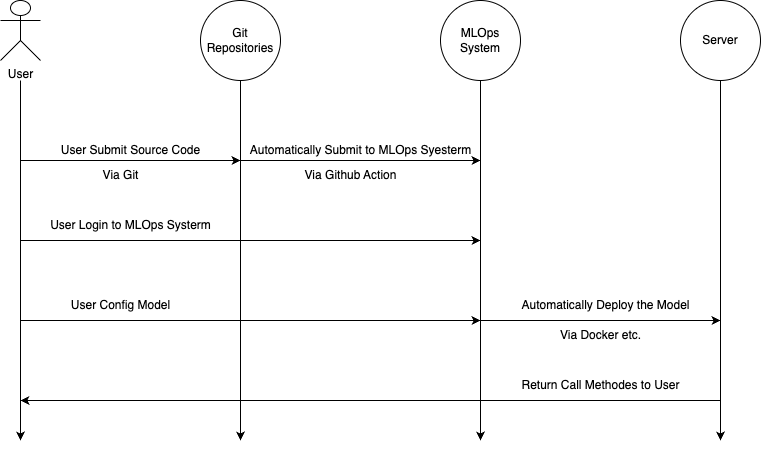
\includegraphics[width=1\textwidth]{P-1.png} %插入图片,[]中设置图片大小,{}中是图片文件名
\caption{时序图} %最终文档中希望显示的图片标题
\label{图片.2-1} %用于文内引用的标签
\end{figure}

开发人员在本地开发机器学习模型,使用Python和TensorFlow等框架设计和训练模型,并将源代码提交到GitHub代码仓库。之后,通过GitHub Action作为CI工具,将GitHub仓库中的最新源代码完成代码质量检查,构建Docker镜像并推送到Docker Hub。

开发人员登录MLOps平台,配置和调整模型。配置完成后,MLOps平台会自动部署该模型到服务器,供生产环境使用。

部署的模型通过接口提供预测服务,并将调用方法返回给用户。用户可以通过接口调用模型服务,发送新数据进行预测和推理。

\subsection{持久化集成技术概述}

技术选型是设计一个MLOps系统的关键步骤之一。其中,持续集成工具的选择尤为重要。持续集成工具能够自动构建和测试代码,极大提高开发效率和软件质量。

本设计选取了GitHub Action作为CI工具。GitHub Action是GitHub提供的持续集成服务,其具有以下优点:

\begin{enumerate}
    \item 无缝集成于GitHub,配置简单,用户体验好。用户可以通过在代码仓库中添加YAML格式的workflow文件来设置CI pipeline,无需登录外部服务或维护额外的服务器。
    \item 丰富的功能,支持构建、测试、发布等一系列CI流程。特别适合基于机器学习的项目,提供了丰富的容器化环境。
    \item 安全稳定,作为GitHub的内置服务,其安全性和稳定性有保障。用户也无需将密钥添加到第三方服务中。
    \item 价格低廉,对公共仓库免费提供所有功能,轻松满足中小项目需求。
\end{enumerate}

相比其他CI服务,如GitLab CI和Travis CI,GitHub Action具有明显优势。GitLab CI虽然功能强大,但其部署较复杂,而Travis CI的价格和技术更新较落后。综合而言,GitHub Action在易用性、丰富的ML功能和体验性价比等方面更胜一筹,更加适合本项目的技术需求。

综上,GitHub Action作为一种简单高效、功能强大的CI服务,完全满足本设计的技术需求。其无缝集成于代码仓库的优点,使得CI流程的配置极为简单方便。特别是对机器学习项目,其丰富的机器学习相关Action和环境,可以最大限度减少配置工作,提高MLOps系统的易用性。

因此,本设计选取GitHub Action作为CI工具,用于实现训练模型的自动化构建、测试和部署流程,是一种理想选择。它可以让研究人员专注于机器学习模型的开发,而不必过多投入到MLOps系统的搭建中,从而大大提高工作效率和研发产出。

\subsection{后端技术概述}

后端技术的选择也是设计一个MLOps系统的关键决定之一。后端框架的高效、稳定对系统性能至关重要。本设计选取Golang语言的Hertz框架作为后端技术。

Hertz是一个Golang HTTP微服务框架。相比其他流行框架如FastAPI和gin,Hertz具有以下优势:

\begin{enumerate} 
    \item 高性能。Hertz参考fasthttp等优秀框架设计,能够实现高并发和低延迟。这对实时性要求高的MLOps系统尤为重要。  
    \item 高扩展性。Hertz的路由、中间件、插件机制灵活高度可定制,可以轻松扩展出满足各种业务场景的解决方案。这使得Hertz非常适合企业级的MLOps产品研发。
    \item 高易用性。Hertz的API设计简单清晰,降低Golang后端学习门槛,方便研发人员快速上手并实现业务需求。
\end{enumerate} 

相比之下,FastAPI作为一个Python框架,性能较差且部署较繁琐。gin虽然也是一个Golang框架,但是扩展性和定制性不如Hertz。综上,Hertz在系统性能、研发效率和实际需求的满足度上更胜一筹,这也是许多公司选择Hertz作为微服务框架的原因。

综上,Hertz是一个高性能、高扩展的Golang HTTP微服务框架,完全满足MLOps系统的技术需求。其简单易用的特性可以让研发人员投入更多精力于业务和模型的开发中,从而提高工作效率。Golang语言天然的并发优势也使得Hertz基于其上开发出的系统,有极高的性能、稳定性和伸缩性。

因此,本设计选择Hertz作为后端框架,用于实现MLOps系统的业务逻辑层。它可以带来高throughput和低延迟,从而满足机器学习模型在线服务的高性能需求。这是实现一套高效智能运维系统的理想基石。

\subsection{前端技术概述}

前端技术的选择也对MLOps系统的用户体验至关重要。本设计选取Next.js框架作为前端主框架,NextUI组件库作为UI解决方案。

Next.js是一个轻量级的React框架,具有以下优势:

\begin{enumerate}   
    \item 简单易用。Next.js大大简化了React应用的配置和部署,降低前端学习门槛,方便开发者快速上手。这可以让开发者投入更多精力于UI和交互的开发中。
    \item 高性能。Next.js内置的静态和服务器端渲染可以实现React应用的高性能交付和部署。这对显示大量机器学习数据和结果的MLOps系统尤为重要。  
    \item 丰富的生态。Next.js与许多UI组件库、状态管理库等有良好的兼容性。这使得Next.js非常适合开发丰富且复杂的MLOps产品。  
\end{enumerate}

相比React仅提供View层的库,Next.js提供了完整的解决方案;相比Vue在渲染方式和性能上略逊一筹。所以,Next.js在易用性、性能和生态上更胜一筹,这也是许多企业选择Next.js开发产品的原因。

NextUI是一套基于Next.js开发的UI组件库。其简洁的视觉风格和丰富的组件可以快速搭建MLOps系统的界面,大幅提高开发效率。

综上,Next.js是一个功能强大且易于上手的React框架,NextUI可以提供配套的UI组件,完全满足MLOps系统的前端需求。它们可以让研发人员专注于交互体验的开发,轻松构建一个简洁高效的用户界面。这是实现一套人性化智能运维系统的理想方案。

因此,本设计选择Next.js作为前端主框架,NextUI作为UI组件库,用于开发MLOps系统的用户界面。它们可以带来良好的用户体验,有力支撑机器学习模型和工具的交互式展示。这是实现人机协同运维的关键一环。

\setcounter{table}{0}
\setcounter{figure}{0}
\clearpage
\section{系统设计}
\subsection{模型侧设计}
\subsubsection{模型的持久化集成设计}

该部分设计旨在探寻如何使用GitHub Action实现模型的持续集成与部署,以实现自动化智能运维、构建高效智能运维平台的需求。具体流程如下:

\begin{enumerate}   
    \item 代码推送到master分支,GitHub Action自动触发。
    \item GitHub Action拉取最新代码。 
    \item GitHub Action设置Python 3.9运行环境,并安装flake8和pytest等依赖。
    \item GitHub Action使用flake8工具检查代码风格和质量。如果检查不通过,则流程终止。
    \item 如果检查通过,GitHub Action使用secrets提供的密码登录Docker仓库。
    \item GitHub Action构建Docker镜像,并推送至Docker仓库,包括自定义的image name和tag。
    \item 至此,持续集成流程完成。每次代码提交,该流程会自动运行,以保证代码的质量和可部署性。
\end{enumerate}

采用持续集成机制可以有效降低人工干预,提高集成效率。GitHub Action提供了全自动化的模型集成过程,大大节省了研发人员的劳动成本和时间。此外,Action使用secrets提供的密码实现Docker登录,解决了密码可能泄露的安全隐患,满足了成熟的MLOps系统对模型管理的需求。

该设计在实现模型的自动构建与部署的同时,降低了研发周期和提高了上线频率,有效支持日益复杂的人工智能算法更新迭代。持续集成机制为构建一个高效智能运维平台奠定了基础,并是实现自动化智能运维的关键之一。

\subsubsection{模型的容器构建设计}

该部分设计旨在探寻如何使用Docker实现模型容器构建,以实现自动化智能运维、构建高效智能运维平台的需求。具体流程如下:

\begin{enumerate}   
    \item 选择Python 3.9-slim作为基础镜像。该镜像体积小且包含Python运行环境,非常适合机器学习模型部署。  
    \item 设置工作目录为/app。这是后续步骤的工作目录。
    \item 复制requirements.txt文件,并安装依赖。这确保容器内含有运行模型所需的所有Python包。
    \item 清理pip缓存和apt缓存,以减小镜像体积。
    \item 复制当前目录.下的全部文件,这会复制模型代码到容器中。 
    \item 暴露端口7007。这是模型服务使用的端口。
    \item 设置容器启动命令为python main.py。这会直接启动模型主入口文件。
\end{enumerate}

至此,Dockerfile构建完成。运行docker build可以构建出模型部署所需的容器镜像。

相比手动配置容器,Dockerfile实现了模型容器的标准化与自动化构建。这简化了部署流程,降低出错概率,有助于实现智能运维的稳定性与连续性。

Docker容器具有以下优点:

\begin{enumerate}   
    \item 隔离性。容器内运行的是独立的操作系统,和主机互不影响,这增强了模型运行的安全性与稳定性。
    \item 轻量级。容器不需要虚拟机,直接利用主机内核,所以体积小和启动时间快。这有利于模型的快速启动与迭代。
    \item 标准化。Dockerfile定义了一个标准的环境和运行命令,每次构建出的容器环境都是一致的。这是多人协作项目的基石。 
    \item 便捷性。Docker简化了环境配置与部署步骤,容器镜像也便于传输与分发。这大大节省了研发人员的时间与精力。
    \item 可扩展性。用户可以在Dockerfile加入更多步骤,也可以配置容器网络、存储等,以适应不同模型和业务场景的需求。  
\end{enumerate}

本设计的Dockerfile构建出的容器镜像,完全满足人工智能模型快速启动与持续更新部署的需要。它通过隔离模型、提供标准环境和简化流程等特性,有效支撑复杂模型在生产环境的稳定运行。这是建立智能运维基础架构的关键。

综上,Docker容器和Dockerfile是实现自动化部署与持续集成的理想技术方案。它们给MLOps系统带来的诸多优势,有力推动了机器学习领域的迭代速度和创新步伐。这是构建人工智能与人的协作代表作的基石。

\subsection{后端侧设计}
\subsubsection{容器管理接口设计}
\paragraph{容器应用数据库设计}

在设计用于管理容器化应用的数据库时,容器应用程序表是核心表之一,它记录了每个容器应用的详细信息。

\begin{table}[htbp]
\caption{容器应用表}
\label{table:app}
\centering
\begin{tabular}{l|l|l}
\hline
\textbf{参数} & \textbf{类型} & \textbf{解释} \\ \hline
app\_id & INT UNSIGNED & 应用ID,自增主键,唯一标识应用 \\
app\_name & VARCHAR(64) & 应用名称,方便用户识别应用\\
app\_status & ENUM & 应用状态,枚举类型,限定为开发中/上线/下线/关闭\\
app\_port & INT & 应用监听端口,INTEGER,需唯一\\
app\_image & VARCHAR(256) & 应用Docker镜像,存储镜像名称+标签\\
user\_id & INT UNSIGNED & 应用所属用户,外键关联Users表\\
is\_deleted & TINYINT(1) & 是否软删除,BOOLEAN,0未删除/1已删除\\
create\_at & DATETIME & 创建时间,时间戳,记录应用注册时间\\
update\_at & DATETIME & 最后更新时间,时间戳,用于跟踪最后修改时间\\
\hline
\end{tabular}
\end{table}

app\_id字段定义为自增主键,用于唯一标识每一个容器应用。作为主键,它可以确保记录的唯一性。

app\_name字段存储应用程序的名称,采用VARCHAR类型以支持较长的名称。应用名称用于方便用户识别和管理不同的应用。

app\_status枚举字段定义应用程序的状态,可以是“开发中”(development)、“上线”(online)、“下线”(offline)或“关闭”(closed)。记录应用的部署状态是管理容器应用的重要部分,枚举类型可以限定状态只能为设定的几种状态。

app\_port字段记录应用程序监听的端口号,用于在主机上映射容器的端口。该端口需要在一台主机上保证唯一,因此定义为UNIQUE。INTEGER类型可以存储数字类型的端口号。

app\_image字段存储应用程序所使用的Docker镜像,用于在主机上创建容器。VARCHAR类型可以存储较长的镜像名称和标签。

user\_id字段记录应用程序所属的用户,用于定义每个应用的所有者和访问控制。通过与Users表的外键关联来定义两表之间的关系。

is\_deleted字段是一个布尔值,用于标记应用程序是否被软删除。TINYINT类型的布尔值,0代表未删除,1代表已删除。

create\_at字段存储应用程序的创建时间,使用DATETIME类型的时间戳记录应用的注册时间。

update\_at字段记录应用程序的最后更新时间,使用DATETIME类型的时间戳在每次更新应用信息时自动更新,用于跟踪应用最后一次的修改时间。

主键约束和外键约束分别定义app\_id的主键约束和user\_id的外键约束,以保证数据表的完整性和一致性。选择InnoDB数据库引擎来支持外键约束。

综上,该应用程序表设计记录了管理容器化应用所需的所有关键数据,包括应用信息、状态、镜像、端口、用户等。它是实现容器应用管理的核心表之一。

该表采用标准的三范式设计,表结构规范,没有数据冗余。这有助于数据的一致性和完整性。同时定义了符合语义的字段,如app\_name、app\_status、app\_image等,名称具有明确的意义。这使得数据库更易于理解和维护。并使用相关的数据类型,如enum枚举类型的app\_status字段。这可以在数据库层面对数据进行约束。外键约束的设置可以保证用户ID的数据完整性,实现表之间的引用完整性。

该表同时有软删除标记和时间戳,使得系统能记录更完整的日志和进行数据恢复。并且枚举字段app\_status创新性的设计为开发中、上线、下线和关闭四种状态。这四种状态能够涵盖容器应用的完整生命周期,更加贴近实际工作流程。

UNIQUE约束的app\_port字段确保在一台主机上应用的端口唯一,防止端口冲突。这是容器应用数据库设计的新增要求。软删除标记is\_deleted使数据库支持应用的软删除,这是容器应用数据库相比一般数据库的新增需求。

Docker镜像存储在app\_image字段,这是容器化应用专有的设计,支持应用部署和上线。

所以,该数据库设计既达到了通用的高质量设计要求,又包含了容器应用管理的一些创新和专属需求,是一套比较完备的容器应用管理数据库方案。

\paragraph{创建应用接口设计}

该设计将实现一个创建应用的接口。

此接口设计将实现接收请求、验证请求、用户认证、应用隔离部署、创建应用记录于数据库的完整逻辑,其中生成未使用端口和通过Docker启动隔离的容器运行应用的方法具有一定创新。

该设计为后续的应用查询、访问、管理、部署等提供了基础,具有完整性和扩展性。同时,该接口也体现了RESTful API的设计理念,请求及响应格式清晰,易于理解。

\paragraph{查询当前用户应用列表接口设计}

此接口设计将实现查询当前登录用户的所有应用列表。

此接口将实现查询当前用户应用列表的功能,为用户提供自己应用的概览,也为其他接口提供查询用户应用的基础。是MLOps系统中用户应用管理的一个关键接口。

通过此接口,用户可以清晰地掌握自己建立的所有应用的基本信息和状态,为后续的应用访问、管理、部署等提供依据。

同时,这个接口也体现了RESTful API的设计理念,请求和相应格式简洁清晰。

\paragraph{更新指定应用信息接口设计}

此接口设计将实现更新指定应用信息的功能,包括应用名称、镜像等。

此接口将实现更新指定应用基本信息和重载应用的功能,使得用户可以灵活管理自己的应用,保证应用可用性,这在MLOps系统的应用管理中具有重要作用。用户可以在此基础上进行应用扩容、配置变更等操作,构建自动化、高可用的机器学习系统。

该函数将实现应用Docker镜像的重载逻辑。它首先通过Docker SDK停止应用已运行的Docker容器。然后拉取最新镜像并启动新容器,映射与旧容器相同的端口,实现无缝重载。

这个函数为应用更新提供了高可用性支持,使应用能够进行零停机重载,这在机器学习系统的运行中至关重要。函数使用Docker SDK实现容器管理,体现了容器化技术的应用。

\paragraph{删除指定应用信息接口设计}

此接口设计将实现软删除指定应用的功能。

此接口将实现软删除指定应用的功能,使得用户可以灵活管理自己的应用,这在MLOps系统的应用管理中具有重要作用。用户可以在此基础上进行应用备份、恢复等操作,构建健壮的机器学习工作流。

软删除的实现使得应用可以实现恢复,比直接物理删除更加灵活和可靠。这体现了数据库管理的高级应用。

总之,此接口设计将实现MLOps系统软删除指定应用的核心功能,为用户应用管理提供重要支撑,具有较高的实用价值和创新性。这也体现了RESTful API的设计理念,请求和响应格式清晰简洁。

\subsubsection{用户管理接口设计}
\paragraph{用户信息数据库设计}

用户表是容器应用管理系统的另一个核心表,它存储用户的账号信息和个人信息。

\begin{table}[htbp]
\caption{用户信息表}
\label{table:user}
\centering
\begin{tabular}{l|l|l}
\hline
\textbf{参数} & \textbf{类型} & \textbf{解释} \\ \hline
user\_id & INT UNSIGNED & 用户ID,自增主键,唯一标识用户\\
user\_name & VARCHAR(32) & 用户名,最大32字符,需唯一\\
email & VARCHAR(64) & 用户邮箱,最大64字符,需唯一\\
password & VARCHAR(256) & 用户密码,最大256字符\\
avatar & VARCHAR(256) & 用户头像URL,可选\\
is\_active & TINYINT(1) & 是否激活,布尔值,0未激活/1已激活\\
is\_admin& TINYINT(1) & 是否管理员,布尔值,0普通用户/1管理员\\
is\_deleted & TINYINT(1) & 是否软删除,布尔值,0未删除/1已删除\\
create\_at & DATETIME & 注册时间,时间戳,记录用户注册时间\\
update\_at & DATETIME & 最后更新时间,时间戳,用于跟踪最后修改时间\\
\hline
\end{tabular}
\end{table}

user\_id字段定义为自增主键,用于唯一标识每个用户。作为主键,它可以确保记录的唯一性。

user\_name字段存储用户名,规定最大长度为32个字符。用户名需要在系统中唯一,所以定义了UNIQUE约束。

email字段存储用户邮箱,规定最大长度为64个字符。用户邮箱也需要在系统中唯一,所以也定义了UNIQUE约束。

password字段存储用户密码,规定最大长度为256个字符。

avatar字段存储用户头像URL,采用VARCHAR类型以支持较长长度。该字段为可选。

is\_active字段是一个布尔值,用于标记用户账号是否被激活。TINYINT类型的布尔值,0代表未激活,1代表已激活。

is\_admin字段也是一个布尔值,用于标记用户是否为管理员账户。0代表普通用户,1代表管理员用户。

is\_deleted字段的布尔值用于标记用户账号是否被软删除。0代表未删除,1代表已删除。

create\_at字段记录用户注册时间,使用DATETIME类型的时间戳。

update\_at字段记录用户信息最后更新时间,使用DATETIME类型的时间戳,在信息更新时自动更新。

PRIMARY KEY定义user\_id字段的主键约束。UNIQUE KEY分别定义user\_name和email字段的唯一性约束。

该用户信息表设计将实现账号管理的基本需求,包含用户注册登录、账户激活和管理、用户数据软删除和权限控制等功能。通过与应用程序表的关系,可以实现用户拥有的应用和权限管理的功能。其标准的三范式设计和相关的数据类型及约束保证了数据的完整性、一致性和质量。

该表同样采用标准的三范式设计,表结构规范,没有数据冗余。这有助于数据的一致性和完整性。同样定义了符合语义的字段,如user\_name、email、password等,名称具有明确的意义。这使得数据库更易于理解和维护。

使用相关的数据类型,如布尔值的is\_active和is\_admin字段使用TINYINT类型。这在数据库层面对数据进行了约束。唯一性约束的设置可以确保用户名和邮箱在系统中唯一,实现业务逻辑需求。同时有软删除标记和时间戳,使得系统能记录更完整的日志和进行数据恢复。

is\_admin字段创新性的定义为是否为管理员用户,用于在系统中实现角色级权限划分,满足实际的应用场景需求。可选的avatar字段可以存储用户头像URL,这是个扩展字段,为系统的功能扩展留出空间。软删除标记is\_deleted使数据库支持用户账号的软删除,这是用户管理数据库相比一般数据库的新增需求。

所以,该用户信息表设计既实现了用户管理的通用需求,又包含了容器应用管理系统的一些专属创新需求,是一套比较完备的用户管理数据库方案。与应用程序表的结合可以满足容器应用管理系统所有的数据需求。

综上,用户表与应用程序表是实现容器应用管理系统的两个核心表,它们相互关联,分别记录系统的用户信息、用户拥有的应用信息和应用状态,能够满足一个高质量容器应用管理系统的关键数据需求。

\paragraph{用户注册接口设计}

此接口设计将实现用户注册功能。

该接口使普通用户可以注册成为系统用户,使用系统提供的各项机器学习应用服务。这也使开发者可以基于用户、用户组等构建复杂的权限管理机制,丰富系统功能。

这体现了RESTful API设计理念的应用,具有良好的模块性和扩展性。

\paragraph{用户登录接口设计}

此接口设计将实现用户登录功能。

该接口使普通用户可以使用用户名与密码登录系统,得到具有一定有效期的JWT token,用于后续接口访问授权。

这使开发者可以基于token实现无状态的接口访问控制,构建RESTful API。

这体现了RESTful API设计理念的应用,具有良好的模块性和扩展性。后续可以在此基础上完善两步验证等安全机制,增强用户信息安全性。

\paragraph{获取当前登录用户信息接口设计}

此接口设计将实现获取当前登录用户信息的功能。

总之,此接口设计简洁高效地实现了获取当前登录用户信息的功能,与用户登录接口配套使用,可以有效减少数据库查询,提高接口性能。

该接口使普通用户可以在登录后,通过此接口快速获取个人信息,用于个人中心等应用场景。这使开发者可以构建无状态的用户信息获取方案,简化系统设计。

这体现了RESTful API设计理念的应用,有利于模块化和接口复用。

\paragraph{邮件管理接口设计}

此接口设计将实现获取验证码的功能。

此接口利用邮件服务实现了获取验证码的功能。这在用户注册和找回密码等场景中很有用。接口返回的响应可以方便前端提示用户验证码已发送。

总之,此接口设计将实现MLOps系统获取验证码的核心功能,与用户注册等接口配套使用,具有较高的实用价值。

该接口使普通用户可以使用注册邮箱获取验证码,完成验证过程。这使开发者可以构建基于邮件服务的用户验证方案。

\subsubsection{其他设计说明}
\paragraph{用户鉴权技术设计}

该设计研究了多种用户鉴权技术,选择一种安全而灵活的方案来对API进行保护。

首先,该设计考虑了基于session的鉴权。这是一种比较常用的鉴权机制。服务端生成一个session id返回给客户端,客户端在每次请求时发送该session id。服务端校验session id的有效性以鉴权用户。这种方案的优点是实现简单,但也存在缺点:

\begin{itemize}   
    \item 需要服务端存储大量session数据,不适合高并发场景; 
    \item session可以被窃取,存在安全隐患;
    \item session不适合跨域场景。
\end{itemize}

其次,该设计考虑了基于token的鉴权,具体为JWT(JSON Web Token)。JWT是一种轻量级的基于token的鉴权机制。工作流程是:

\begin{enumerate}   
    \item 客户端使用用户名和密码请求登录;
    \item 服务端校验用户名和密码,登录成功后签发一个JWT;
    \item 客户端在每次请求时使用该JWT进行鉴权;  
    \item 服务端校验JWT的有效性和权限进行鉴权。
\end{enumerate}

这种方案的优点是:

\begin{itemize}
    \item 无状态,利于扩展;  
    \item 安全可靠; 
    \item 方便跨域。
\end{itemize}

因此,该设计最终选择JWT作为我的用户鉴权机制。

\paragraph{容器管理技术设计}

Docker是一个开源的应用容器引擎,使用Go语言开发。Docker可以将应用程序及其依赖打包在一个可移植的容器中,然后在任何支持Docker的Linux或Windows环境中运行。

Docker go sdk是Docker官方提供的Golang语言编程接口。使用Docker go sdk可以很方便地在Golang应用程序中管理Docker资源,如镜像、容器等。因此,在本MLOps系统中选择Docker go sdk作为容器管理技术,具有以下优点:

\begin{enumerate}   
    \item 官方支持。Docker go sdk由Docker公司开发和维护,稳定性和兼容性都有保证,使用风险较小。
    \item 简单易用。Docker go sdk提供了一系列简洁的Golang API,开发人员可以很容易地管理Docker资源,编写Docker相关逻辑。 
    \item 高性能。Docker go sdk底层用C语言实现,并作了高度优化,性能较高。此外,由于Go语言自身的高性能,使用Docker go sdk开发的程序也具有较好性能。
    \item 跨平台。由于Docker和Golang同为跨平台技术,基于Docker go sdk开发的程序可以运行在不同操作系统的物理机或虚拟机上。
\end{enumerate}

综上,Docker go sdk作为Docker的官方Golang语言SDK,具有官方支持、简单易用、高性能和跨平台等优点。使用Docker go sdk可以非常方便和高效地管理Docker资源,是容器管理技术的不错选择,适用于本MLOps系统的需求。

\subsection{前端侧设计}
\subsubsection{官网页设计}

该官网页面将采用Next.js框架设计实现。

主要样式使用styled-components实现,通过tagged template literals语法扩展并创建新的HTML标签,这体现了组件化和模块化设计思想。页面路由使用Next.js的文件系统路由,方便快速构建。

该部分使用组件和模块化开发网页。这使网页结构清晰,各部分独立,扩展性强。

主要布局使用Box和Layout两个组件实现。Box为页面的main部分提供一个灵活布局。这使主体部分样式统一又易于修改。

使用styled-components为组件开发定制样式。这使样式与组件结合,组件的可重用性强。并通过创建新的HTML标签扩展样式。

\subsubsection{登录页设计}

该登录页将采用Next.js框架设计实现。

登录流程如下:

\begin{enumerate}
\item 点击登录链接,打开模态框 
\item 在模态框中填入邮箱和密码
\item 点击提交,调用登录API 
\item 如果成功,获取用户信息,跳转到dashboard页面,关闭模态框
\item 如果失败,提示登录失败,模态框不关闭该登录页
\end{enumerate}

该页面采用函数组件和Hooks设计。这使页面结构清晰,且易于理解和扩展。并且主要通过Modal和Input两个组件构建登录表单。这使表单清晰精简,Modal组件使其以弹出框形式出现。同时使用useState管理模态框visible和表单values状态。

这实现了组件状态的管理。该登录页设计简洁高效,采用相应组件实现登录表单和流程,与API对接完成登录功能,并提供必要的用户交互提示。

\subsubsection{注册页设计}

该登录页将采用Next.js框架设计实现。

注册流程如下:

\begin{enumerate}
\item 点击注册链接,打开模态框
\item 在模态框中填入用户名、邮箱、密码和验证码
\item 点击发送验证码,调用API发送验证码到邮箱
\item 输入收到的验证码,点击提交
\item 调用注册API,如果成功,自动调用登录API并跳转到dashboard页面,关闭模态框
\item 如果失败,提示注册失败,模态框不关闭
\end{enumerate}

该注册页采用函数组件和Hooks设计。这使页面结构清晰,且易于理解和扩展。主要通过Modal和Input两个组件构建注册表单。这使表单清晰精简,Modal组件使其以弹出框形式出现。使用useState管理模态框visible和表单values状态。

这实现了组件状态的管理。调用发送验证码、注册和登录API,与后端对接。这实现了注册和登录功能的核心逻辑。注册成功后通过router跳转到dashboard页面。

这实现了注册后的页面切换。ModalFooter中包含关闭、发送验证码和提交按钮。这提供了用户交互方式。

\subsubsection{模型提交页设计}

该登录页将采用Next.js框架设计实现。

提交流程如下:

\begin{enumerate}
\item 在Card组件中填入模型名称和Docker镜像
\item 点击提交按钮,调用创建模型API
\item 如果成功,跳转到列表页,页面刷新
\item 如果失败,页面不跳转,表单值不清空
\end{enumerate}

该模型提交页采用函数组件和Hooks设计。这使页面结构清晰,且易于理解和扩展。主要通过Card和Input两个组件构建模型提交表单。这使表单清晰简洁,Card提供包裹容器。

使用useState管理表单values状态。这实现了组件状态的管理。调用创建模型API与后端对接。这实现了模型提交的核心逻辑。

提交成功后通过router跳转到列表页。这实现了页面之间的导航和刷新。Button组件提供提交按钮。这实现了用户交互方式。Flex和Grid组件用于页面布局。这使页面结构灵活清晰。

\subsubsection{模型列表页设计}

该登录页将采用Next.js框架设计实现。

列表流程如下:

\begin{enumerate}
\item 调用getAppAPI获取模型列表,存储在models状态中
\item 用Table组件循环渲染models,其中操作和状态列使用RenderCell组件渲染
\item RenderCell组件根据columnKey选择对应渲染组件,包含User、StyledBadge、Text等
\item 操作列包含编辑UpdateModel、删除DeleteModel和查看模型功能
\end{enumerate}

该模型列表页采用函数组件和Hooks设计。这使页面结构清晰,且易于理解和扩展。

主要通过Table、User和StyledBadge组件构建模型列表页面。这使列表简洁清晰,Table提供列表容器。

调用获取模型API与后端对接。这实现了模型列表的核心功能。RenderCell自定义渲染组件实现操作和状态列功能。这增加了列表的交互性。UpdateModel和DeleteModel组件实现编辑和删除模型功能。这增强了列表的可操作性。Flex和Grid组件用于页面布局。

这使页面结构灵活清晰。useState和useEffect管理用户、模型列表和重载状态。这实现了组件状态的管理。

\setcounter{table}{0}
\setcounter{figure}{0}
\clearpage
\section{系统实现}
\subsection{模型侧实现}
\subsubsection{模型的持久化集成实现}
该部分配置文件如下:

{\noindent}\rule[0pt]{15cm}{0.05em}
\begin{verbatim}
name: Python CI and Docker Image Build
on:
  push:
    branches:
      - master
jobs:
  build:
    runs-on: ubuntu-20.04
    steps:
    - name: Checkout code
      uses: actions/checkout@v2
    - name: Set up Python environment
      uses: actions/setup-python@v2
      with:
        python-version: 3.9
    - name: Install dependencies
      run: |
        pip install --upgrade pip
        pip install flake8 pytest
    - name: Lint code with flake8
      run: |
        flake8 .
    - name: Login to Docker Registry
      run: echo "${{ secrets.DOCKER_PASSWORD }}" | 
            docker login -u "${{ secrets.DOCKER_USERNAME }}" 
            --password-stdin
    - name: Build and Push Docker Image
      run: |
        docker build -t lyleshaw/gradio-test -f ./Dockerfile .
        docker push lyleshaw/gradio-test:latest
\end{verbatim}
{\noindent}\rule[0pt]{15cm}{0.05em}

\subsubsection{模型的容器构建实现}

该部分DockerFile如下:

{\noindent}\rule[0pt]{15cm}{0.05em}
\begin{verbatim}
FROM python:3.9-slim
WORKDIR /app
COPY requirements.txt ./
RUN pip install --upgrade pip \
    && pip install --no-cache-dir -r requirements.txt \
    && rm -rf /root/.cache/pip \
    && rm -rf /var/lib/apt/lists/*
COPY . .
EXPOSE 7007
ENTRYPOINT ["python", "main.py"]
\end{verbatim}
{\noindent}\rule[0pt]{15cm}{0.05em}

\subsection{后端实现}
\subsubsection{容器管理接口实现}
\paragraph{创建应用接口实现}

创建应用的接口实现如下:

CreateApp接口实现了接收创建应用请求,验证请求,获取请求用户信息,生成应用端口,启动Docker镜像,创建应用记录于数据库的完整流程。

其中,生成端口函数GeneratePort通过随机算法生成未使用的端口,避免端口冲突,这是创新点之一。

启动Docker镜像函数StartDockerImage通过Docker SDK拉取指定镜像并启动容器,映射端口以供外部访问,这实现了应用的隔离运行,是创新点之二。

创建应用记录CreateApplication将应用信息写入数据库,以供后续查询和管理。

CreateApp接口接收来自前端的创建应用请求req,包含应用名称AppName、镜像名称AppImage等信息。接口首先验证请求数据,然后从请求上下文c中获取当前登录用户信息user。接着,GeneratePort生成一个未使用的端口port供应用使用。

然后,StartDockerImage函数通过Docker SDK拉取req中指定的AppImage镜像,并启动一个容器,映射port端口以供外部访问。这个容器的ID记录在container中。

最后,CreateApplication函数将名称AppName、端口port、镜像AppImage、Docker容器IDcontainer.ID以及user的用户ID用户信息录入数据库,创建应用记录。

CreateApplication函数将应用信息结构化为models.Application,并使用GORM库将其写入MySQL数据库。记录了应用名称AppName、端口AppPort、镜像AppImage、Docker容器IDDockerID、创建用户的userID、应用状态AppStatus和删除标志IsDeleted。

\paragraph{查询当前用户应用列表接口实现}

此接口设计实现了查询当前登录用户的所有应用列表。

MyApp接口接收来自前端的查询请求req,并从请求上下文c中获取当前登录用户信息user。然后,GetApplicationsByUserID函数Uses GORM查询数据库,获取userID对应的所有应用记录apps。

GetApplicationsByUserID函数使用GORM的Where条件,过滤IsDeleted为false(未删除)的应用记录,找到userID对应的所有应用。如果查询失败,函数会返回对应错误信息err。

MyApp接口将查询得到的[]∗model.Application类型的应用记录apps转换为[]∗service.Application类型的响应格式respApps。最后构造service.AppListResp响应,包含code、message及data,通过c.JSON返回给请求方。

\paragraph{更新指定应用信息接口实现}

UpdateApp接口接收来自前端的更新应用请求req,包含应用IDAppID、应用名称AppName、镜像AppImage及是否重载IsReload等信息。接口首先根据AppID查询指定应用信息application,然后验证请求用户user是否为该应用的创建用户。

如果req.IsReload为真,接口会通过ReloadDockerImage函数重载应用的Docker镜像。

该函数将实现应用Docker镜像的重载逻辑。它首先通过Docker SDK停止应用已运行的Docker容器。然后拉取最新镜像并启动新容器,映射与旧容器相同的端口,实现无缝重载。

这个函数为应用更新提供了高可用性支持,使应用能够进行零停机重载,这在机器学习系统的运行中至关重要。函数使用Docker SDK实现容器管理,体现了容器化技术的应用。

最后,UpdateApplicationByID函数使用GORM更新application记录,如果req中包含新名称AppName和镜像AppImage,则进行更新。并重新查询最新application,构造响应resp返回。

ReloadDockerImage和UpdateApplicationByID函数分别实现了应用镜像重载和数据库更新的具体逻辑。ReloadDockerImage通过Docker SDK停止旧容器并启动新容器实现应用重载,这一操作对用户而言是透明的,也避免了应用停顿,具有较高的可用性。

\paragraph{删除指定应用信息接口实现}

DeleteApp接口接收来自前端的删除应用请求req,包含应用ID AppID。接口首先根据AppID查询指定应用信息application,然后验证请求用户user是否为该应用的创建用户。

验证通过后,StopDockerImage函数使用Docker SDK停止应用运行的Docker容器,并移除容器。

最后,DeleteApplicationByID函数使用GORM更新application记录,将IsDeleted字段置为true,实现软删除。并构造响应resp返回。

StopDockerImage函数实现了应用Docker容器的停止和移除操作,释放了应用使用的计算资源。DeleteApplicationByID函数实现了应用软删除的数据库操作,将应用的IsDeleted标记为已删除,但保留应用记录,这在应用恢复功能中很有用。

此外,StopDockerImage函数的实现展示了Docker技术在机器学习系统中的应用,实现了应用容器的高效管理。这是构建MLOps系统的关键技术之一。

\subsubsection{用户管理接口实现}
\paragraph{用户注册接口设计}

Register接口接收来自前端的用户注册请求req,包含用户名Username、邮箱Email、密码Password及验证码Code等信息。

接口首先验证req.Code是否与内存中的邮箱对应的验证码匹配,以完成邮箱验证。然后调用CreateUser函数实现用户注册的数据库操作。

CreateUser函数使用GORM创建用户记录user,用户密码Password通过HashAndSaltPassword函数哈希加密后存储,提高安全性。如果创建成功,函数返回user及nil错误,否则返回对应错误信息err。

Register接口根据CreateUser的返回值构造响应resp,包含code、message及data(user),通过c.JSON返回给请求方。

此接口设计将实现用户注册的完整流程,是构建用户认证体系的基石。CreateUser函数的密码加密操作也提高了用户信息安全性,这在用户密码管理中很有价值。

接口及CreateUser函数都使用context.Context作为第一个参数,这体现了Context设计理念的应用,使得接口具有较好的容错性和扩展性。

总之,此接口设计实现了MLOps系统用户注册的核心功能,为构建用户认证授权体系提供基础,具有较高的安全性、实用价值和扩展性。

\paragraph{用户登录接口实现}

Login接口接收来自前端的用户登录请求req,包含用户名Username、密码Password等信息。接口首先调用GetUserByEmail函数根据req.Email查询用户记录user。然后使用utils.ComparePasswords函数比较req.Password与user.Password是否匹配。

如果比对成功,接口使用jwt.NewWithClaims函数生成包含user信息的JWT token,并设置过期时间。

最后构造响应resp,包含code、message、data(token及expire),通过c.JSON返回给请求方。GetUserByEmail和ComparePasswords函数分别实现了根据邮箱查询用户和密码比对的具体逻辑。jwt.NewWithClaims函数使用JWT实现了用户身份认证与授权的功能,这在用户认证体系中至关重要。

此接口设计将实现用户登录的完整流程与JWT token的颁发,是构建用户认证体系的关键接口。密码比对的实现也提高了用户信息安全性,这在用户登录管理中很有价值。接口使用context.Context作为第一个参数,这体现了Context设计理念的应用,使得接口具有较好的容错性和扩展性。

总之,此接口设计将实现MLOps系统用户登录的核心功能,为构建用户认证授权体系提供关键支撑,具有较高的安全性、实用价值和扩展性。

\paragraph{获取当前登录用户信息接口实现}

GetUser接口首先从请求context中获取key为mw.IdentityKey的用户信息user。如果user不存在,则返回401未授权状态码。

如果user存在,则构造响应resp,包含code、message及data(user信息)。通过c.JSON返回给请求方。

此接口利用JWT token在登录成功后嵌入的用户信息,实现无状态的用户信息获取。这体现了RESTful API设计理念的应用,具有良好的扩展性。

此接口使用context.Context作为第一个参数,这体现了Context设计理念的应用,使得接口具有较好的容错性和扩展性。

\paragraph{邮件管理接口设计}

SendCode接口首先从请求req中获取email,并进行校验。如果校验失败,返回400状态码。
如果校验成功,接口调用utils.SendEmail函数向email发送验证码。如果发送失败,返回500状态码。

如果发送成功,构造响应resp,包含code和message,通过c.JSON返回给请求方。

SendEmail函数实现了具体的发送邮件逻辑。它从环境变量中获取邮件服务器配置,生成随机验证码,构建邮件内容,最后通过mail.NewDialer连接邮件服务器并发送。

接口使用context.Context作为第一个参数,这体现了Context设计理念的应用,使得接口具有较好的容错性和扩展性。并使用c.BindAndValidate进行参数校验,这提高了接口健壮性。

\subsection{前端侧实现}
\subsubsection{官网页实现}

主要组件与最终成果图如下:

\begin{table}[htbp] 
\caption{官网页组件表}   
\label{table:landingPage}
\centering
\begin{tabular}{c|c}
\hline
\textbf{组件} & \textbf{功能}\\ 
\hline
Nav  & 顶部导航栏组件,提供页面内导航功能\\
\hline
Layout & 页面布局组件,包含Nav,负责页面整体框架\\   
\hline
Hero & 首页英雄图部分,用于主视觉区\\
\hline  
Box & 一个灵活的布局组件,这里作为main标签使用\\
\hline
Faq & 页面中部的常见问题部分\\
\hline
Footer & 页脚组件\\
\hline
\end{tabular}
\end{table}

\begin{figure}[H] %H为当前位置,!htb为忽略美学标准,htbp为浮动图形
\centering %图片居中

\includegraphics[width=1\textwidth]{P-2.png} %插入图片,[]中设置图片大小,{}中是图片文件名
\caption{官网页} %最终文档中希望显示的图片标题
\label{图片.landing} %用于文内引用的标签
\end{figure}

\subsubsection{登录页实现}

主要组件与最终成果图如下:

\begin{table}[htbp] 
\caption{登录页组件表}   
\label{table:login}
\centering
\begin{tabular}{c|c}
\hline
\textbf{组件} & \textbf{功能}\\ 
\hline
Modal & 模态框组件,包含登录表单\\
\hline
Input & 输入框组件,用于邮箱和密码   \\
\hline  
Button & 按钮组件,提交和关闭模态框\\ 
\hline
Checkbox & 复选框组件,用于记住我\\
\hline
useState & React hooks,用于管理模态框和表单值的状态\\
\hline 
loginAPI & 调用登录API,提交表单\\
\hline
getUserAPI & 获取用户信息API\\
\hline
router & 路由控制,登录成功后跳转\\
\hline 
toast & 提示组件,登录失败提示\\
\hline
\end{tabular}
\end{table}

\begin{figure}[H] %H为当前位置,!htb为忽略美学标准,htbp为浮动图形
\centering %图片居中
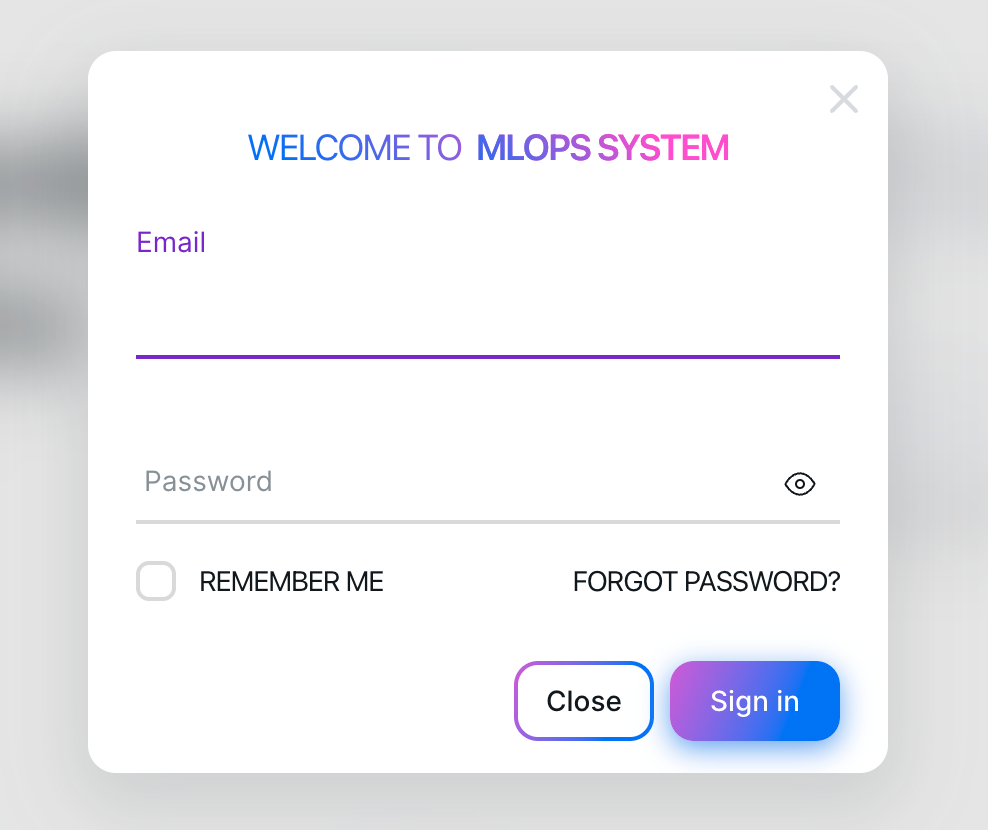
\includegraphics[width=1\textwidth]{P-3.png} %插入图片,[]中设置图片大小,{}中是图片文件名
\caption{登录页} %最终文档中希望显示的图片标题
\label{图片.login} %用于文内引用的标签
\end{figure}

\subsubsection{注册页实现}

主要组件与最终成果图如下:

\begin{table}[htbp] 
\caption{注册页组件表}   
\label{table:register}
\centering
\begin{tabular}{c|c}
\hline
\textbf{组件} & \textbf{功能}\\ 
\hline
Modal & 模态框组件,包含注册表单\\
\hline
Input & 输入框组件,用于用户名、邮箱、密码和验证码\\
\hline  
Button & 按钮组件,发送验证码、提交和关闭模态框\\ 
\hline
Row和Col & 栅格布局组件,用于验证码输入和发送部分\\
\hline
useState & React hooks,用于管理模态框和表单值的状态\\
\hline 
sendVerificationCodeAPI & 调用发送验证码API\\
\hline
registerAPI & 调用注册API,提交表单\\
\hline
loginAPI & 调用登录API,注册成功自动登录\\
\hline
router & 路由控制,注册成功后跳转\\
\hline 
toast & 提示组件,注册失败提示\\
\hline
\end{tabular}
\end{table}

\begin{figure}[H] %H为当前位置,!htb为忽略美学标准,htbp为浮动图形
\centering %图片居中
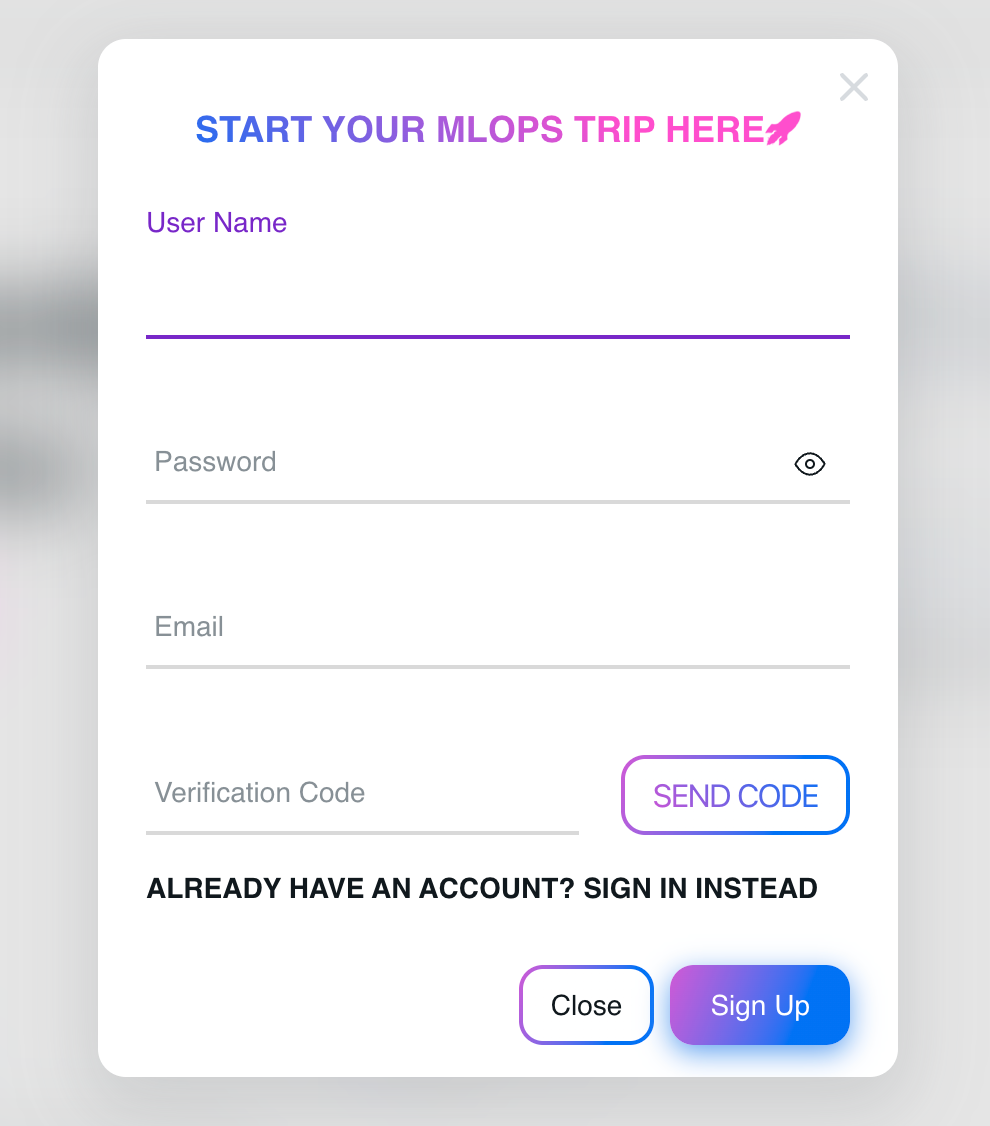
\includegraphics[width=1\textwidth]{P-4.png} %插入图片,[]中设置图片大小,{}中是图片文件名
\caption{注册页} %最终文档中希望显示的图片标题
\label{图片.register} %用于文内引用的标签
\end{figure}

\subsubsection{模型提交页实现}

主要组件与最终成果图如下:

\begin{table}[htbp] 
\caption{模型提交页组件表}   
\label{table:submit}
\centering
\begin{tabular}{c|c}
\hline
\textbf{组件} & \textbf{功能}\\ 
\hline
Flex和Grid & 布局组件,用于页面整体布局\\
\hline
Input & 输入框组件,用于模型名称和Docker镜像\\
\hline  
Button & 按钮组件,提交表单\\ 
\hline
Card & 组件,用于包含模型提交表单\\
\hline
useState & React hooks,用于管理表单值的状态\\
\hline 
createAppAPI & 调用创建模型API,提交表单\\
\hline
router & 路由控制,提交成功后跳转到列表页\\
\hline 
\end{tabular}
\end{table}

\begin{figure}[H] %H为当前位置,!htb为忽略美学标准,htbp为浮动图形
\centering %图片居中
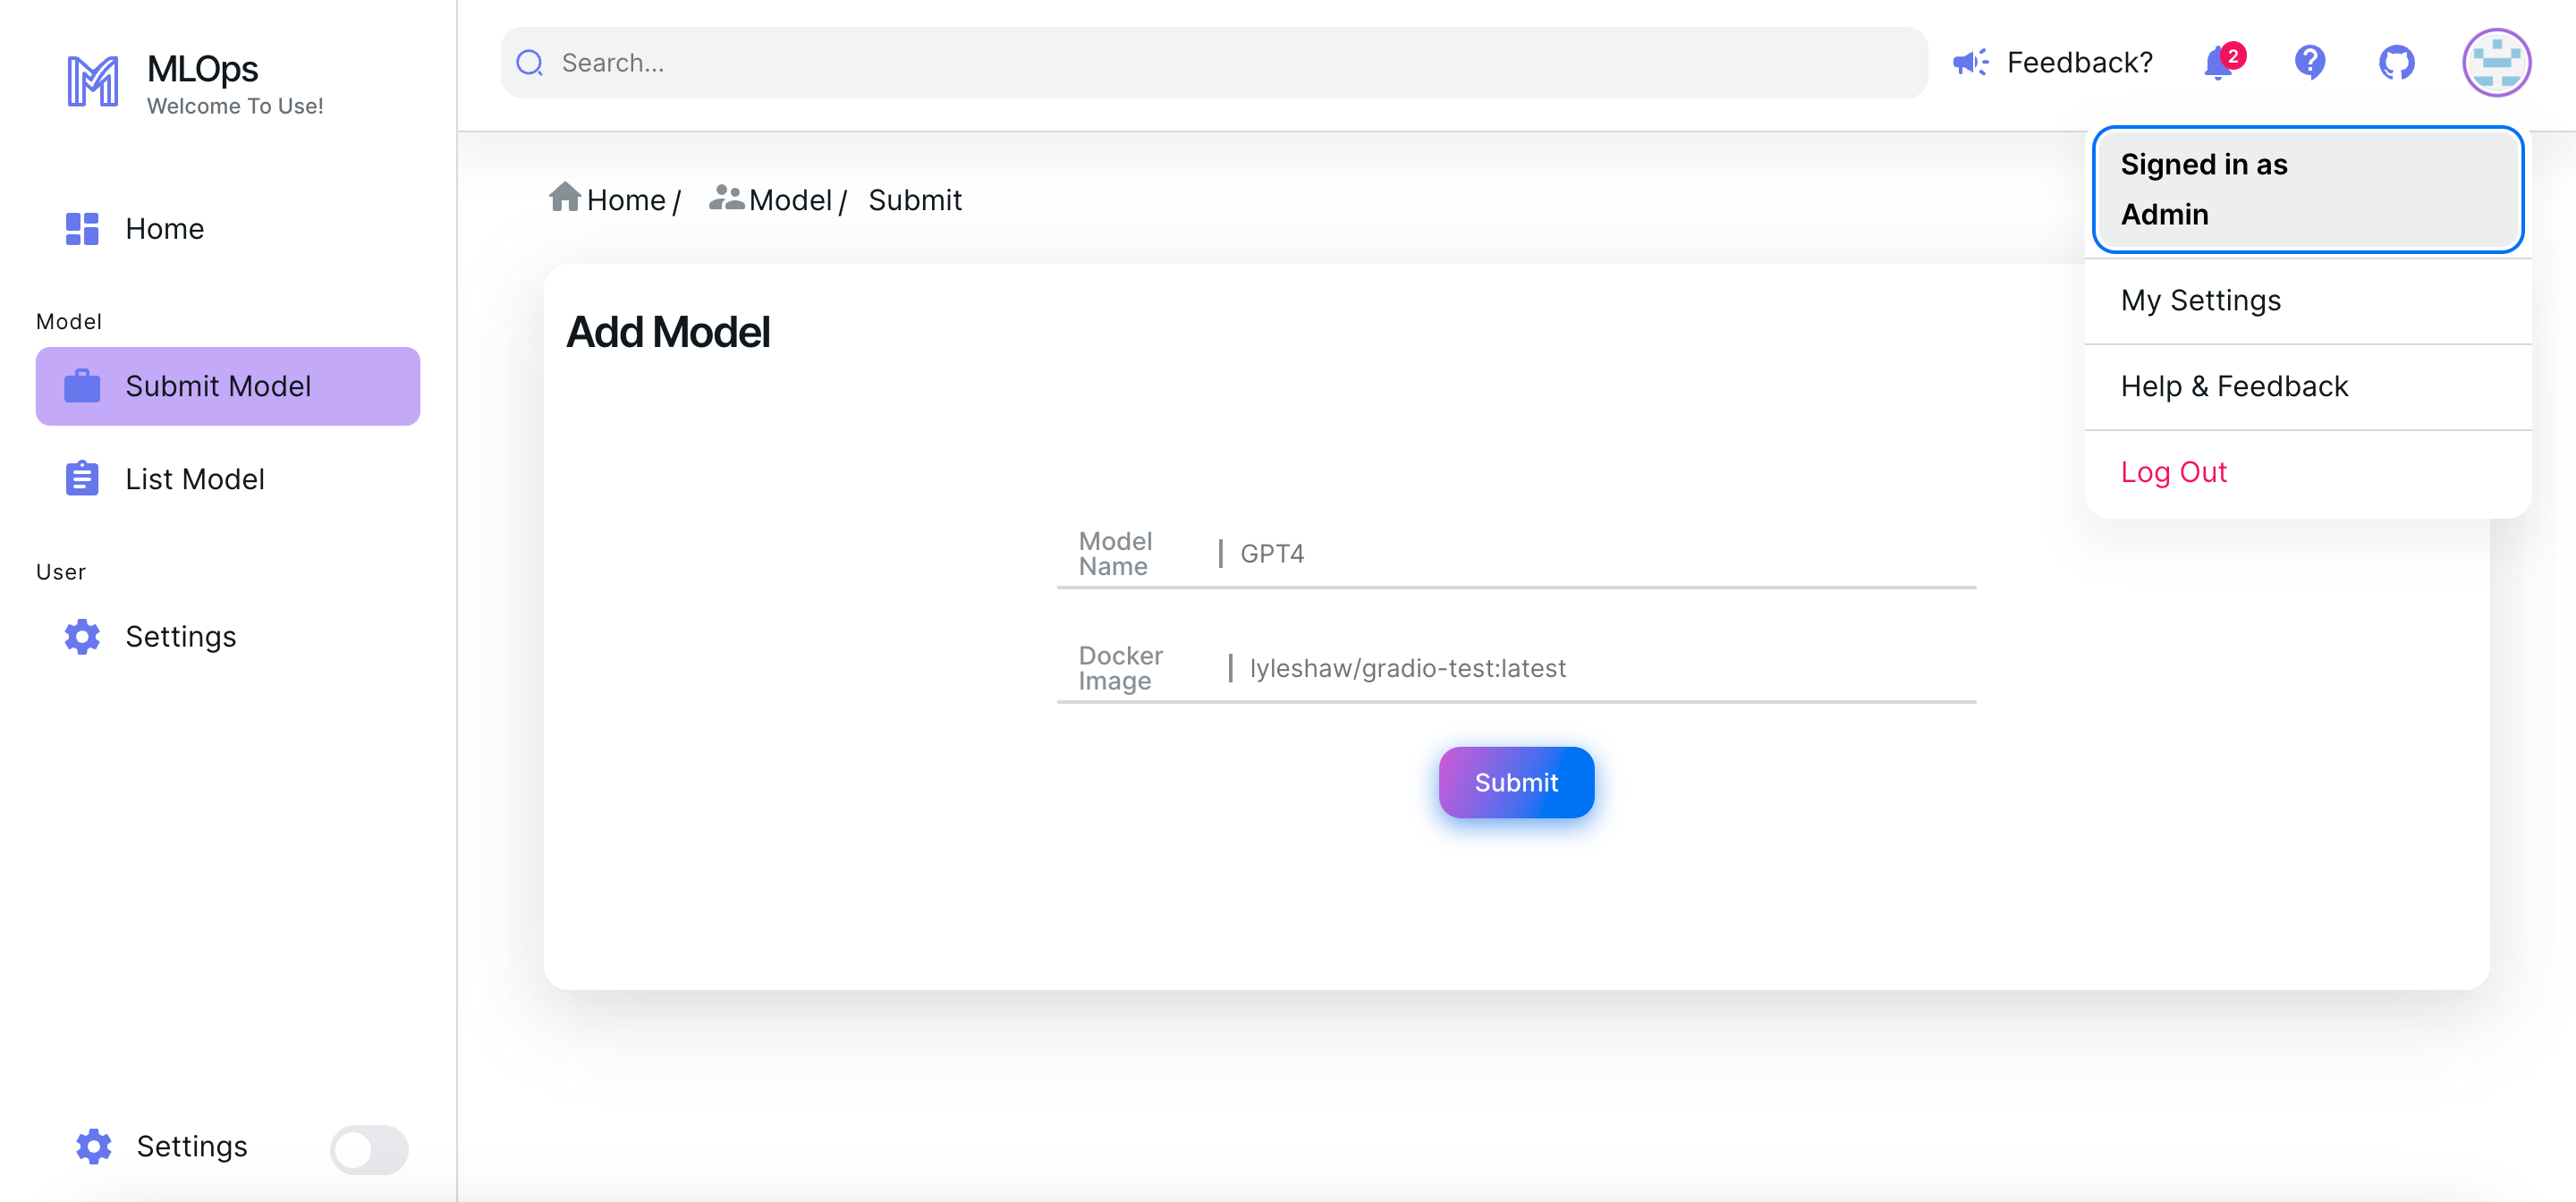
\includegraphics[width=1\textwidth]{P-5.png} %插入图片,[]中设置图片大小,{}中是图片文件名
\caption{模型提交页} %最终文档中希望显示的图片标题
\label{图片.submit} %用于文内引用的标签
\end{figure}

\subsubsection{模型列表页实现}

主要组件与最终成果图如下:

\begin{table}[htbp]
\caption{模型列表页组件表}  
\label{table:list}
\centering
\begin{tabular}{c|c}
\hline
\textbf{组件} & \textbf{功能}\\ 
\hline
Flex和Grid & 布局组件,用于页面整体布局\\
\hline
Card & 组件,用于包含模型列表\\
\hline
Input & 搜索输入框组件\\
\hline 
Button & 添加模型按钮组件\\
\hline
Table & 表格组件,用于显示模型列表\\ 
\hline
useState和useEffect & React hooks,用于管理用户、模型列表\\
\hline
getAppAPI & 调用获取模型API,获取模型列表\\
\hline
RenderCell & 自定义单元格渲染组件,用于操作和状态列\\
\hline
User、StyledBadge & 组件,用于操作列渲染\\
\hline
UpdateModel和DeleteModel & 组件,用于操作列编辑和删除模型功能\\
\hline
router & 路由控制,未登录跳转到登录页\\
\hline
\end{tabular}
\end{table}

\begin{figure}[H] %H为当前位置,!htb为忽略美学标准,htbp为浮动图形
\centering %图片居中
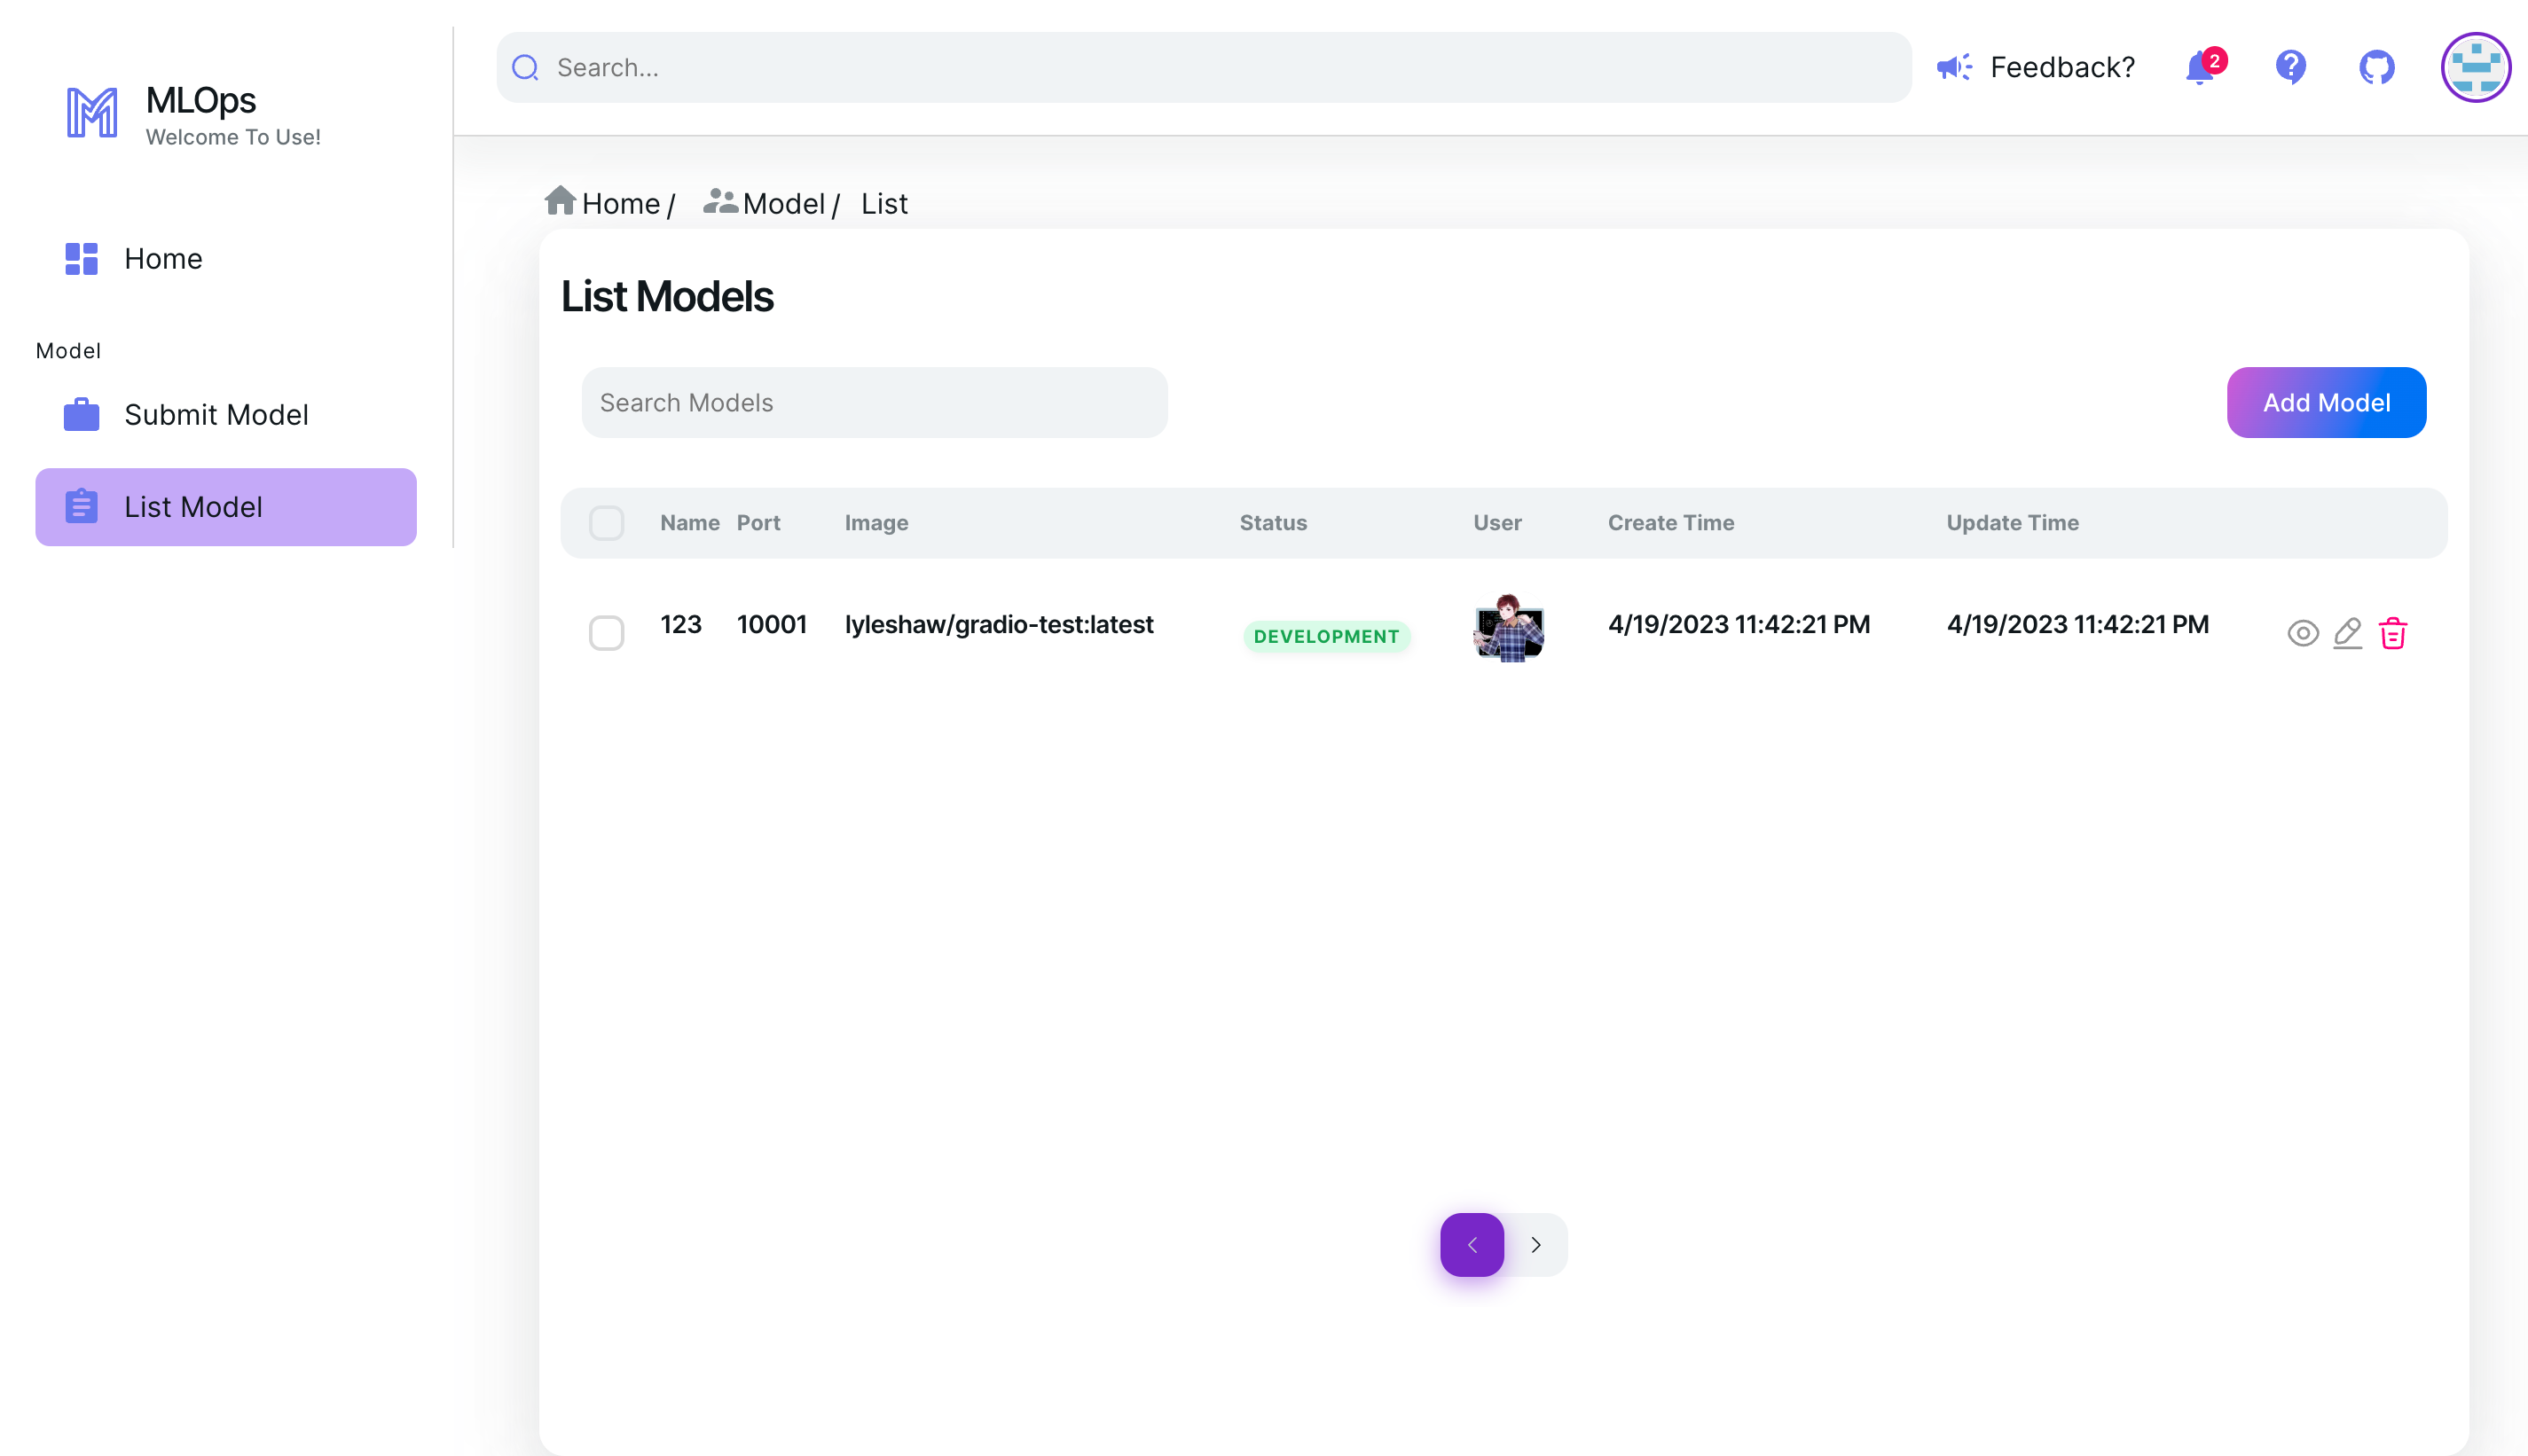
\includegraphics[width=1\textwidth]{P-6.png} %插入图片,[]中设置图片大小,{}中是图片文件名
\caption{模型列表页} %最终文档中希望显示的图片标题
\label{图片.list} %用于文内引用的标签
\end{figure}

\setcounter{table}{0}
\setcounter{figure}{0}
\clearpage
\section{测试与部署}
\subsection{单元测试}
\subsubsection{容器部分单元测试}

本部分定义了三个测试函数来进行Docker镜像的单元测试,分别是:

TestStartDockerImage:该函数首先通过调用StartDockerImage()启动一个Docker镜像,然后检验返回的containerInfo是否正确,包括containerID不为空以及其他信息。最后调用StopDockerImage()停止刚启动的镜像。该测试函数的目的是验证StartDockerImage()函数正常启动Docker镜像的功能。

TestStopDockerImage:该函数直接调用StartDockerImage()启动一个Docker镜像,然后调用StopDockerImage()停止该镜像。测试的目的是独立验证StopDockerImage()函数停止Docker镜像的功能是否正常。

TestReloadDockerImage:该函数首先调用StartDockerImage()启动一个Docker镜像,然后调用ReloadDockerImage()函数重载该镜像,最后调用StopDockerImage()停止该镜像。该测试函数的目的是验证ReloadDockerImage()函数重载Docker镜像的功能是否正常。

这三个测试函数的执行可以有效验证Docker容器管理的三个关键功能,分别是:启动Docker镜像、停止Docker镜像以及重载Docker镜像。通过这三个功能的测试,可以确保Docker容器管理系统的稳定性、健壮性,并在功能发生变更时快速发现问题,达到提高软件质量和减少维护成本的目的。

单元测试的主要意义是确保每个功能单元(函数或模块)的正确性和鲁棒性,这三个测试函数的设计使得Docker容器管理系统的三个核心功能得以被有效测试和验证。这种基于功能的单元测试设计方法,有利于后续维护和开发,不会由于系统变更导致这三个关键功能产生错误,真正发挥了单元测试的价值。总之,这部分测试函数在提升容器管理部分代码稳健性、鲁棒性和可维护性上发挥了重要的作用。

\subsubsection{应用数据库操作部分单元测试}

该代码定义了应用数据库操作的单元测试,主要测试了以下功能:

\begin{enumerate}   
    \item 创建应用:TestCreateApplication()函数测试创建应用的功能,检验创建后应用的各个字段是否正确。
    \item 根据用户ID获取应用:TestGetApplicationsByUserID()函数先创建两个应用,然后根据用户ID获取这两个应用,并检验获取的应用信息是否正确。
    \item 根据ID获取应用:TestGetApplicationByID()函数先创建一个应用,然后根据应用ID获取该应用,并检验获取的应用信息是否正确。
    \item 根据ID更新应用:TestUpdateApplicationByID()函数先创建一个应用,然后根据应用ID更新应用名称和镜像,并检验更新后应用的名称和镜像是否正确。 
    \item 根据ID更新应用状态:TestUpdateApplicationStatusByID()函数先创建一个应用,然后根据应用ID更新应用状态,并检验更新后应用的状态是否正确。
    \item 根据ID删除应用:TestDeleteApplicationByID()函数先创建一个应用,然后根据应用ID删除该应用,并检验应用是否被正确标记为已删除。
    \item 生成应用端口:TestGeneratePort()函数先调用GeneratePort()生成一个端口,检验生成的端口是否正确,然后创建一个应用占用该端口,再次调用GeneratePort()生成一个新的端口,检验生成的端口是否正确。
\end{enumerate}

这些测试函数涵盖了应用数据库操作的主要功能,可以有效验证这些功能的正确性,确保应用数据库的稳定可靠运行。同时,这些测试也具有导向作用,可以指导数据库操作相关功能的设计与实现。总之,这些测试对提高应用数据库操作系统的质量有重要作用。

这部分代码实现的应用数据库操作测试,与第一部分的Docker容器测试一样,都属于功能测试的一种——单元测试。这种测试方法有利于软件的可维护性与扩展性,是现代软件工程中重要的质量保障手段。

\subsubsection{用户数据库操作部分单元测试}

这部分代码定义了用户数据库操作的单元测试,主要测试了以下功能:

\begin{enumerate}   
    \item 创建用户:TestCreateUser()函数测试创建用户的功能,检验创建后用户的各个字段是否正确。
    \item 根据ID获取用户:TestGetUserByID()函数先创建一个用户,然后根据用户ID获取该用户,并检验获取的用户信息是否正确。   
    \item 根据邮箱获取用户:TestGetUserByEmail()函数先创建一个用户,然后根据用户邮箱获取该用户,并检验获取的用户信息是否正确。
    \item 获取所有用户:TestGetAllUsers()函数先创建两个用户,然后获取所有用户,并检验获取的用户数量和信息是否正确。
    \item 根据ID更新用户:TestUpdateUserByID()函数先创建一个用户,然后根据用户ID更新用户名、邮箱和密码,并检验更新后用户的信息是否正确。
    \item 根据ID删除用户:TestDeleteUserByID()函数先创建一个用户,然后根据用户ID删除该用户,并检验用户是否被正确标记为已删除。 
\end{enumerate}

这些测试函数涵盖了用户数据库操作的主要功能,可以有效验证这些功能的正确性,确保用户数据库的稳定可靠运行。同时,这些测试也具有导向作用,可以指导用户数据库操作相关功能的设计与实现。总之,这些测试对提高用户数据库操作系统的质量有重要作用。

这部分测试采用的也是单元测试方法,与前两部分的测试一致。单元测试是软件测试中比较基础而重要的方法,可以最大限度地提高软件的稳定性、可靠性和可维护性。这三个部分的测试共同构成了整个系统的测试体系,有效保障了系统的高质量。

通过学习和分析这三个部分的测试代码,可以了解单元测试和功能测试的常用方法与思想。熟练掌握这些测试方法,对个人技能提高和软件开发质量保障都大有裨益。总之,测试是现代软件工程中不可或缺的一部分,值得软件开发者投入时间和精力学习与实践。

\subsection{部署方案}

整个系统的部署分为后端部署和前端部署两个部分。

后端部署采用如下方案:

\begin{enumerate}
    \item 后端代码部署在自有云服务器上,服务器配置为2核4G内存,系统为Ubuntu 20.04。
    \item 在服务器上安装Docker,用于管理和运行各个应用对应的Docker镜像。Docker 可以有效隔离不同应用环境,方便应用的部署和管理。
    \item 使用cloudflare tunnel为后端应用提供公网访问,实现前后端的通信。云服务cloudflare tunnel可以快速为应用提供全球覆盖的访问,不需要服务器进行复杂的端口映射和安全配置。
    \item 后端应用监听cloudflare tunnel分配的域名和端口,接收来自前端的请求并返回相应的数据。  
\end{enumerate}

前端部署采用如下方案:

\begin{enumerate}
    \item 前端代码使用NextJS框架开发,部署在Vercel平台上。Vercel是NextJS官方推荐的部署和托管平台,可以快速免费部署NextJS应用。
    \item 前端应用需要访问的后端接口使用cloudflare tunnel分配的域名。请求被发送到cloudflare,再被重定向到后端服务器上对应应用。
    \item 前后端使用RESTful API进行接口通信。前端发送HTTP请求到后端接口,后端返回JSON格式的数据。
\end{enumerate}

综上,本系统采用前后端分离的部署方案。这种方案可以充分利用云服务的便利,同时也可以避免被云服务厂商的技术和价格锁定,有利于系统的长期运行。这是一种开源与云服务相结合的部署思路,可以作为小型应用部署的较佳实践。

\setcounter{table}{0}
\setcounter{figure}{0}
\clearpage
\section{总结与展望}

本设计方案达到了任务书的要求,成功设计并实现一套MLOps系统来自动化完成从模型发布到模型应用的工作流。

工作流的内容包括:

\begin{enumerate}
    \item 开发者发布生产环境的模型到Git代码仓库。
    \item 通过自动化的CI工作流对仓库的代码质量和安全性进行检查,确保模型的正确性和安全可靠。 
    \item 对模型进行打包,生成对应的Docker镜像。
    \item 系统接收到Docker镜像的URL,将模型部署到生产环境。
\end{enumerate}

同时完成了对整套系统的单元测试与冒烟测试,确保所有功能模块可以正常稳定运行。

这次毕业设计对我来说既是一个机遇,也是一个挑战:

通过本次毕业设计,我学习到了许多新知识,增强了动手实践的能力。实际工作中遇到的各种问题需要我仔细分析并逐步解决,这大大提高了我的实践能力与解决问题的思维能力。

通过实际的工程设计,我认识到书本知识与实际应用之间的差异。实践中涉及到的技术细节远比书本内容丰富得多,这需要我在设计与开发过程中不断学习和进步。

本次毕业设计是我第一次参与较大型软件系统的全流程设计与开发,既是一个难得的学习机会,也是一个巨大的挑战。我通过努力不断克服各种困难,最终成功完成了系统设计与开发,这大大增强了我的信心与决心。

总之,本次毕业设计使我在知识与能力上有了很大提高,这将为我今后的学习与工作打下良好的基础。我将继续努力,在软件设计与开发的道路上不断前行。

\clearpage
\unnumberedsection{致谢}{致\hspace{2em}谢}

首先,我要感谢我的指导老师陈溪源老师。在毕业设计的所有阶段,陈溪源老师给予我的指导和支持对我非常的重要并使我受益匪浅。

其次,我要感谢计算机科学与技术专业的各位老师,在本学期开课过程中,老师们精心准备的课件和教案使我学习到了许多宝贵的知识,这些知识为我的毕业设计打下了良好的基础。其中尤其要感谢秦飞巍老师,没有他的创新实践课程对我的启发,就不会有我的毕业设计的想法。

最后,我要感谢我的朋友和家人,在我撰写毕业论文的过程中,他们给予我的支持和鼓励,使我有动力完成这篇论文。

在此,请允许我再次表达我对各位老师和朋友的衷心感谢,没有你们的帮助,我无法完成本篇论文,谢谢你们!

\clearpage
% 修正目录超链接问题
\phantomsection{}
% 列出参考文献
% \printbibliography[heading=bibintoc]

\unnumberedsection{参考文献}

\begin{thebibliography}{99}
\bibitem{ref1}王一沛,刘庭辉.基于机器学习的运维数据分析系统设计与研究[J].电子技术与软件工程,2022(21):259-262.
\bibitem{ref2}黄伟.基于机器学习的AIOps技术研究[D].北京交通大学,2019.DOI:10.26944/d.cnki.gbfju.2019.000297.
\bibitem{ref3}施育军.基于Spark的AIOps系统的设计与实现[D].厦门大学,2020.DOI:10.27424/d.cnki.gxmdu.2020.000942.
\bibitem{ref4}陈立忠.基于机器学习的智能化自动化运维[J].中国新通信,2020,22(14):44-46.
\bibitem{ref5}孙宇峰,李锐.商业银行信息系统自动化运维的研究与实践[J].金融电子化,2018(09):82-84.
\bibitem{ref6}袁红团.基于云计算智能电网安全运维管理系统设计与研究[J].自动化与仪器仪表,2021(06):120-122+127.DOI:10.14016/j.cnki.1001-9227.2021.06.120.
\bibitem{ref7}Monika Steidl. The Pipeline for the Continuous Development of Artificial Intelligence Models -- Current State of Research and Practice[EB/OL]. 2023[2023]. https://doi.org/10.48550/arXiv.2301.09001.
\bibitem{ref8}Shawn Hymel. Edge Impulse: An MLOps Platform for Tiny Machine Learning[EB/OL]. 2022[2023]. https://doi.org/10.48550/arXiv.2212.03332.
\bibitem{ref9}Dominik Kreuzberger. Machine Learning Operations (MLOps): Overview, Definition, and Architecture[EB/OL]. 2022[2023]. https://doi.org/10.48550/arXiv.2205.02302.
\bibitem{ref10}G. Symeonidis. MLOps -- Definitions, Tools and Challenges[EB/OL]. 2022[2023]. https://doi.org/10.48550/arXiv.2201.00162.
\bibitem{ref11}Cedric Renggli. A Data Quality-Driven View of MLOps[EB/OL]. 2021[2023]. https://doi.org/10.48550/arXiv.2102.07750.
\end{thebibliography} 

\clearpage
\unnumberedsection{附录}{附\hspace{2em}录}

\end{document}